\begin{comment}
Algoritmo exacto para clases de equivalencias en “árboles”
    Forma Naive
    Cálculo de clases de equivalencia para cada unrelated tree
    Combinar clases de los unrelated tree con ancestros y descendientes
        Combinación con descendientes
        Combinación con ancestros
    Complejidad total
        Complejidad de #UnrEC
        Complejidad de #eqClass
        Complejidad total del algoritmo
\end{comment}

Nuestro objetivo es computar $\assym_{M,e,\Pr}(x_i)$ dado un grafo causal $G$ (que es un DAG). Recordemos que:

$$\assym_{M,e,\Pr}(x_i) = \heuristicASVFormula$$

%\santi{Agregar paréntesis a los primeros términos de la sumatoria.}

Una forma de obtener este valor es calculando primero el conjunto de clases de equivalencia $eqCl(G, x_i)$, para luego tomar un representante de cada una (es decir, un orden topológico), con el cual evaluar la expresión dentro de la sumatoria. 
%\santi{Usar referencias a Figuras y no decir ``a continuación'' o ``En el grafo de abajo''.}

\subsection{Solución Naive} \label{alg:naiveAlgorithmEquivalenceClass}

%\santi{Capaz esto puede ir antes del dibujo anterior y la descripción, como una forma sencilla de calcular $eqCl(G, x_i)$. Después proponés la idea de calcular las clases de equivalencia mediante combinaciones de subclases de equivalencia.}

La manera más sencilla de obtener las clases y sus representantes consiste en: calcular todos los órdenes topológicos del bosque utilizando algún algoritmo de generación de los mismos \cite{KNUTH1974153}. Luego, iterar sobre los ordenes topológicos y asignarles a una clase de equivalencia, en base a cuáles nodos no relacionados están antes de $x_i$. Una vez hecho esto, tendremos nuestras clases, un representante para cada una de ellas y sus tamaños. El problema de este algoritmo es que necesitamos calcular explícitamente cada orden topológico de $G$, lo cual puede ser $O(n!)$ en el peor caso, ya que esa es la cota para todos los ordenes topológicos posibles.

\subsection{Algoritmo recursivo}

%\santi{Es raro este subtítulo porque hace parecer que el algoritmo Naive no es exacto.}

En este trabajamos proponemos un algoritmo recursivo para calcular las clases de equivalencia sin calcular explícitamente todos los órdenes topológicos. El algoritmo para encontrar este conjunto de clases se divide en dos partes: en la primera obtenemos las clases de equivalencia para los árboles no relacionados (es decir, aquellos subárboles que contienen nodos que no son ni descendientes ni ancestros de $x_i$), y en la segunda fusionamos estas clases con los ancestros y descendientes. En la Figura~\ref{fig:ASV_forest_example} podemos ver como  quedan etiquetados los distintos nodos:

\begin{figure}[H]
    \centering
    \begin{tikzpicture}[scale=.65, transform shape, 
    unrelated/.style={circle, draw=red},
    ancestor/.style={circle, draw=blue},
    wiggly/.style={decorate, decoration={snake, amplitude=.2mm, segment length=2mm}}  % Define wiggly line style
    ]
        \node[text=blue] at (-5, 0) {Ancestors};
        \node[text=teal] at (-5, -0.5) {Descendants};
        \node[text=red] at (-5, -1) {Unrelated};        
        
        % ---- NODOS ----

        \node[ancestor] (a1) at (0, 0) {$a_1$};
        \node[unrelated] (u1) at (-1, -2) {$u_1$};
        \node[ancestor] (a2) at (1, -2) {$a_2$};

        \drawUnrelatedTree{u2}{-1}{-4}{$u_2$}
        \node[ancestor] (a3) at (1, -4) {$a_3$};
        \node[unrelated] (u3) at (3, -4) {$u_3$};

        \drawUnrelatedTree{u4}{0}{-7}{$u_4$}
        \node[ancestor] (a4) at (3, -6) {$a_4$};

        \node[nodo] (xi) at (3, -8) {$x_i$};

        \drawUnrelatedTree{r1}{6}{0}{$u_5$} 
        \drawUnrelatedTree{r2}{10}{0}{$u_6$} 
        
        \node[draw=none, fill=none] (hi) at (3, -10) {};


         \path [->] (a1) edge[arista]  (u1);
         \path [->] (a1) edge[arista]  (a2);

         \path [->] (a2) edge[arista]  (u2);
         \path [->] (a2) edge[arista]  (a3);
         \path [->] (a2) edge[arista]  (u3);

         \path [->] (a3) edge[arista]  (u4);
         \path [->] (a3) edge[arista]  (a4);

         \path [->] (a4) edge[arista]  (xi);      
         \path [->, teal] (xi) edge[arista,  decorate, decoration={snake, amplitude=.4mm, segment length=4mm, post length=1mm}] node[right] {descendants of $x_i$} (hi);
    \end{tikzpicture}
    \caption{Ejemplo de un grafo causal $G$, con sus respectivas etiquetas en base a $x_i$}
    \label{fig:ASV_forest_example}
\end{figure}

% \santi{Hace falta este dibujo? No podemos linkear al anterior que es idéntico?} Rta: Para mi hace falta porque tiene los nodos bien etiquetados y esta completo, es la referencia de  se etiquetan. 

\subsubsection{Clases de equivalencia para árboles unrelated}

Sea $UR$ (unrelated roots) el conjunto de nodos que son raíces de un árbol no relacionado. Formalmente, $ur \in UR$ sii $ur$ es una raíz y un nodo no relacionado, o el padre de $ur$ es un ancestro de $x_i$ y $ur$ no es un ancestro de $x_i$. El algoritmo se ejecutará sobre cada una de estas raíces para obtener las clases de equivalencia de estos subárboles. Cada clase de equivalencia puede representarse con un conjunto $\equivalenceClassRep$, como vimos en la Definición \ref{equivalenceClassDefinition}. 

%\santi{No se entiende lo de ``si es una raiz''}
%\santi{No entiendo a qué te referís con representación. Creo que es más adecuado decir que una clase de equivalencia es una función $f$ de los nodos unrelated a $\{left, right\}$.} 

%\echu{Definir esto antes, no puede ser que esto recién aparezca acá. Esto es la forma de identificar  dos órdenes pertenecen a la misma clase de equivalencia}

Nuestro algoritmo devolverá un conjunto de tuplas con el formato $(\equivalenceClassRep, leftTopos, rightTopos)$, donde $leftTopos$ es el número de órdenes topológicos que podemos generar con los nodos no relacionados previos a $x_i$, y $rightTopos$ lo mismo, pero con los que están después. El tamaño de la clase $\equivalenceClass$ se puede calcular mediante esta tupla como $leftTopos * rightTopos$.\\

%\santi{En el fondo es medio confuso que usas la misma notación $[\pi]R$ para denotar clases de equivalencia y también para su ``representación''.}

Para la fórmula a continuación, dado un nodo $n \in V$ notamos como $n_i$ al $i-$ésimo hijo de $n$, y como $|n|$ a su número de hijos. La Ecuación\footnote{Pueden encontrar este algoritmo en \path{\pasantia-BICC\asvFormula\classesSizes\recursiveFormula.py}} \ref{formula:unrelated_equiv_classes} calcula todas las clases de equivalencia posibles en un árbol no relacionado, dada la raíz del mismo. Aplicándola sobre cada nodo $ur \in UR$, obtendremos el conjunto de clases de equivalencia para cada subárbol no relacionado con $x_i$. La función $\unrEqCl(n)$ consiste en obtener todas las clases de equivalencias de los hijos del nodo $n$, para luego unificar cada combinación posible de las mismas. El caso base es cuando $n$ es una hoja, ahí sólo hay dos opciones: $n$ puede estar a la derecha o a la izquierda, y va a tener un sólo orden topológico. 

\begin{align}\label{formula:unrelated_equiv_classes}
    \unrEqCl(n) = 
    \begin{cases} 
    \set{(\set{n_l}, 1, 1), (\set{n_r},1,1)} & \text{si $n$ es una hoja} \\[1ex]
    \begin{aligned}
    &\left( \bigcup_{\forall mix \in \unrEqCl(n_1) \times \dots \times \unrEqCl(n_{|n|})} \hspace{-6em} \union(mix,n_{left})\right) \\
    &\cup \union(right,n_{right})
    \end{aligned} & \text{cc}
    \end{cases}
\end{align}

%\santi{Acá hay un tema de notación, o estoy entendiendo todo mal: $\union$ toma un nodo y una tupla de la forma $(\equivalenceClass, L(\equivalenceClass), R(\equivalenceClass))$ por cada hijo de $n$. Con esta info, hay una \textbf{única} clase de equivalencia que podés armar en la que $n$ esté a la izquierda de $x_i$ y se cumplan las clases de cada uno de los hijos. Si es asi, el problema notacional viene de que vos estás escribiendo $eqCl_j$ para denotar estas clases de los hijos, cuando $eqCl$ denotaba el conjunto de clases de equivalencia. Si estoy en lo cierto, estaría bueno declarar las aridades de las funciones para que sea más fácil entenderlas. El \union también está flojo de papeles. Capaz podemos escribir todo lindo en la próxima reunión. Además estaría bueno agregarle una explicación/semántica a la función (tipo para n que hace), y explicar que devuelve. } Rta: Ahí modifique el texto y la función. 

%\santi{Me parece que la mejor forma de escribir esto sería simplemente contar la relación recursiva de los conjuntos y listo, mandamos al apéndice esta función. Tratemos de escribirlo bien la próxima reunión. También, tratemos de elegir mejores nombres, $UnrEC$ es muy largo.}
La función \textit{union} nos sirve para combinar las distintas clases de equivalencia de cada subárbol, para una explicación más detallada de la misma pueden ir al apéndice a la sección \ref{subsubSection:auxiliaryFormulasUnrelatedTrees}. Para tener una intuición respecto a la correctitud de la función, se pude observar que hay una correspondencia directa entre las clases de equivalencia de un nodo y las de sus hijos. Dado un nodo $n$, cada clase de equivalencia que lo incluye puede descomponerse de manera única en una combinación de clases de equivalencia de sus hijos. Análogamente, si conocemos todas las clases de equivalencia posibles de los hijos de $n$, podemos combinarlas para reconstruir todas las clases de equivalencia de $n$. Esta biyección es la que permite realizar el proceso recursivo definido en la ecuación \ref{formula:unrelated_equiv_classes}.

Por fuera de la unión, tenemos una clase de equivalencia más, la cuál tiene al nodo $n$ a la derecha de $x_i$. Utilizamos $right$ pues es la única unión de clases de equivalencia en la cual todos sus nodos aparecen después de $x_i$, y si $n$ está a la derecha, entonces todos sus descendientes deben estar a la derecha también. Observar que $right$ pertenece al mismo producto cartesiano generado en la unión. %\santi{No se a que se refiera la última oración, la sacaría.} Rta: Se explico en persona
%\echu{Falta esto: "Agregar un parrafito explicando que hay una biyección entre cómo podes -> a través de una clase del padre inferir la de los hijos y cómo a través de las de los hijos podes mezclarlas y obtener la de los padres. " pero no sabría donde meterlo}
%Así se define $right$: \\  $right \in \unrEqCl(n_1) \times \dots \times \unrEqCl(n_{|n|}), \forall (repEC, \_ , \_) \in right, L(repEC) = 0$ \\ Lo saco y no lo pongo porque no tiene mucho sentido
%\santi{Ok, hoy lo escribimos. Quedó medio suelto el $right$, no se cual es tu objetivo.} Lo flete, no pega mucho con la onda de la sección

\paragraph{Optimizaciones}\label{slight_improvement}

Más adelante en este algoritmo vamos a tener que combinar cada uno de nuestros árboles no relacionados con los ancestros, esa parte del proceso es la más costosa en tiempo. Por lo tanto, nuestro objetivo es terminar con la menor cantidad de subárboles para combinar. En base a esta idea, encontramos esta optimización. Imaginemos que tenemos los resultados para $\unrEqCl(ur_1)$ y $\unrEqCl(ur_2)$. Si $ur_1$ y $ur_2$ tienen el mismo padre o ambos son raíces, entonces los vamos a unificar. El procedimiento es análogo a agregar un nodo virtual $v$ en la Figura \ref{fig:ASV_forest_example}, que es el padre de $u_5$ y $u_6$, y luego ejecutamos $\unrEqCl$ desde este nodo, utilizando únicamente el $\union$ (ya que este nodo no existe y nunca podría estar a la derecha de $x_i$). De esta forma sólo vamos a tener cómo máximo un árbol no relacionado por cada ancestro de $x_i$. Otra forma más visual de interpretar esta optimización es que en vez de correr nuestro algoritmo sobre cada $ur$, lo vamos a ejecutar sobre cada ancestro $a$. Teniendo el cuidado de no recorrer, el eje que conecta al ancestro $a$ a $x_i$.
%\santi{No entendí cuál es la optimización expliacada acá.} 
%\echu{¿Ahora se entiende más la idea?}
%\santi{Si. Pero, ¿No es equivalente decir que se ejecuta el algoritmo desde cada ancestro? Teniendo el cuidado de no recorrer, al ejecutarlo sobre un cierto ancestro $a$, el eje que lo acerca a $x_i$ (o sea, el eje que va a otro ancestro). }

\begin{comment}
    Al pedo esta figura, igual que la anterior
    
\begin{figure}[H]
    \centering
    \begin{tikzpicture}[scale=.65, transform shape, 
    unrelated/.style={circle, draw=red},
    ancestor/.style={circle, draw=blue},
    wiggly/.style={decorate, decoration={snake, amplitude=.2mm, segment length=2mm}}  % Define wiggly line style
    ]

        \node[ancestor] (a1) at (0, 0) {$a_1$};
        \node[unrelated] (u1) at (-1, -2) {$u_1$};
        \node[ancestor] (a2) at (1, -2) {$a_2$};

        \drawUnrelatedTree{u2}{-1}{-4}{$u_2$}
        \node[unrelated] (u3) at (3, -4) {$u_3$};

        \drawUnrelatedTree{u4}{0}{-7}{$u_4$}
        \node[ancestor] (a4) at (3, -6) {$a_3$};

        \node[nodo] (xi) at (3, -8) {$x_i$};

        \drawUnrelatedTree{r1}{6}{0}{$u_5$} 
        \drawUnrelatedTree{r2}{10}{0}{$u_6$} 
        
        \node[draw=none, fill=none] (hi) at (3, -10) {};


         \path [->] (a1) edge[arista]  (u1);
         \path [->] (a1) edge[arista]  (a2);

         \path [->] (a2) edge[arista]  (u2);
         \path [->] (a2) edge[arista]  (u3);

         \path [->] (a2) edge[arista]  (u4);
         \path [->] (a2) edge[arista]  (a4);

         \path [->] (a4) edge[arista]  (xi);      
         \path [->, teal] (xi) edge[arista,  decorate, decoration={snake, amplitude=.4mm, segment length=4mm, post length=1mm}] node[right] {descendants of $x_i$} (hi);
    \end{tikzpicture}
    \caption{En este caso, los nodos que unificaríamos con esta optimización son $u5$ y $u6$ pues ambos son raíces, y $u2$ y $u4$ pues comparten un padre.}
    \label{fig:equivClass_optimization_example}
\end{figure}

\end{comment}

\subsubsection{Fusión de clases de unrelated trees con ancestros y descendientes}

Ahora nuestro objetivo es combinar las clases obtenidas previamente con los ancestros y descendientes de $x_i$. ¿Por qué no podemos usar la fórmula anterior y simplemente combinarlas como hacíamos antes? Imaginemos que lo hacemos y usamos directamente $\union$ con los ancestros. La tupla que los representa sería  $(\set{ a_l | a \in A}, 1, 1)$, $A$ = $ancestros$. Esto se debe a que solo tienen un orden posible, y todos ellos deben aparecer antes de $x_i$. Ahora bien, si usáramos $\union$, estaríamos haciendo el cálculo $\binom{|A| + |U|}{|A|}$, lo que significa que podríamos insertar los elementos de $A$ entre cualquier elemento de $U$ (nodos no relacionados) en el orden topológico, ¡pero eso es incorrecto! Porque en este escenario, hay dependencias entre los nodos. En la Figura \ref{fig:ASV_forest_example} no podemos poner $u_1$ antes de $a_1$ o ninguno de los nodos en el subárbol de $u_2$ antes de $a_2$. Esto significa que necesitamos otra función para calcular los órdenes posibles de los nodos que aparecen antes de $x_i$ y los ancestros. Vamos a llamar a esta función $leftOrders$. \\

Ahora la pregunta es, ¿qué hacemos con los descendientes? Aquí no estamos restringidos como lo estábamos antes con los ancestros, por lo que podemos usar una fórmula similar a la del algoritmo \ref{for:topoCountingDTrees}, porque no hay dependencias entre los nodos de $D$ y $UR$. Teniendo esto en cuenta, finalmente podemos definir nuestra fórmula\footnote{Pueden encontrar este algoritmo en \path{\pasantia-BICC\asvFormula\classesSizes\recursiveFormula.py}} \ref{formula:equiv_classes_sizes}. Dado un \dtree{} $G$, un nodo $x_i \in V(G)$, $ur_i$ la raíz del $i-$ésimo árbol no relacionado, $A$ y $D$ los ancestros y descendientes, respectivamente, de $x_i$ en $G$. Utilizando las funciones $eqCl$ y $\eqClassSize$, las cuáles nos devuelven la representación de la clase $\equivalenceClassRep$ y el tamaño de la clase, respectivamente. Con estas funciones auxiliares, las cuáles están definidas en el apéndice en la sección \ref{subsubSection:auxiliaryFormulasEquivalenceClasses}, la fórmula para calcular todas las clases de equivalencia y sus tamaños en $G$ es:

%\echu{Pasar esta formula a una definición y aclarar todas las variables y letras que aparecen + especificar la notación falopa}

\begin{align}\label{formula:equiv_classes_sizes}
    \eqClassSizes(G, x_i) = 
    \bigcup_{\forall mix \in \unrEqCl(ur_1) \times \dots \times \unrEqCl(ur_{|UR|})} \left( eqCl(A,D, mix) , \eqClassSize(A,D,mix) \right) 
\end{align}

%\santi{No diría que esto es una definición.} Concuerdo

\subsubsection{Combinando los ancestros y los nodos no relacionados}

Estas son las variables que vamos a tomar en cuenta para calcular las combinaciones: los $ancestros$, el valor de $L(eqCl)$ (la cantidad de nodos a la izquierda en la clase de equivalencia) para cada $eqCl$ de cada unrelated tree, y la raíz de cada árbol no relacionado. Lo que queremos hacer es definir el número de órdenes topológicos que podemos generar, combinando los nodos a la izquierda de cada unrelated tree con los ancestros. Veamos un ejemplo con el grafo de la Figura \ref{fig:ASV_forest_example}. ¿Qué ordenes topológicos podemos generar con los ancestros posicionados como vemos en la Figura \ref{fig:order_of_ancestors}?

\begin{figure}[ht]
    \centering
    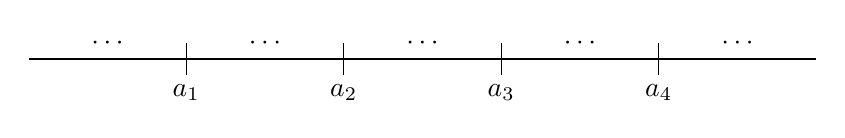
\begin{tikzpicture}
        % Draw the main line
        \draw[thick] (0,0) -- (10,0);
        
        % Draw and label the points
        \foreach \x/\label in {2/$a_1$, 4/$a_2$, 6/$a_3$, 8/$a_4$} {
            \pgfmathsetmacro{\xnew}{\x-1}
            \node at (\xnew,0.2) {$\cdots$};
            \draw (\x,0.2) -- (\x,-0.2); % Ticks
            \node[below] at (\x,-0.2) {\label}; % Labels
        };

    \node at (9,0.2) {$\cdots$};
    \end{tikzpicture}
    \caption{Posible orden topológico con los ancestros ya colocados}
    \label{fig:order_of_ancestors}
\end{figure}

Ahora la pregunta es, ¿dónde podemos colocar los elementos de cada unrelated tree? Antes de $a_1$, solo podemos colocar nodos que estén en los subárboles de $u_5$ o $u_6$. Antes de $a_2$, podemos colocar los mismos elementos, más $u_1$. En general, antes de un nodo $a_i$ podremos colocar todos los nodos que estén incluidos en un $unrelated \ tree$ que tenga como raíz $ur$, tal que $ur$ sea una raíz, o $a_j$ sea el padre de $u_r$ con $j<i$. Ahora queremos convertir esto en una fórmula recursiva, ya que habrá una superposición de problemas utilizamos programación dinámica al implementar el algoritmo. La fórmula más detallada la pueden encontrar en el apéndice en la sección \ref{subsubSection:leftOrdersImplementation}, este es el algoritmo para contabilizar las combinaciones posibles entre los nodos no relacionados y los ancestros:\\

\begin{algorithm}
\caption{leftOrders($A$, $\textit{actual ancestor}$, $\textit{nodes to place}$, $position$)} \label{alg:leftOrdersAlgorithm}
\begin{enumerate}
    \item Definimos donde colocar $\textit{actual ancestor}$ en base a $position$ y a cuántos nodos tenemos disponibles en $\textit{nodes to place}$, generando $\textit{new position}$.
    \item Luego seleccionamos cuántos nodos de cada unrelated tree vamos a usar para llenar todas las posiciones entre $position$ y $\textit{new position}$, generando $\textit{new nodes}$.
    \item Eliminamos los $\textit{new nodes}$ de los $\textit{nodes to place}$, puesto que ya los colocamos, actualizando nuestros nodos disponibles.
    \item Realizamos el llamado recursivo actualizando la posición, nuestros nodos disponibles y nuestro ancestro actual. 
\end{enumerate}
\end{algorithm}

\subsection{Complejidad del algoritmo}
%\echu{ ¿Esta es la idea? ¿Cuánto más formal debería ser? ¿Cuánto mejor lo debería escribir? }
Sea $n$ el número de nodos del digrafo causal $G$, $r$ la raíz de $G$ y $equivalenceClasses$ el conjunto de clases de equivalencia en $G$ para el feature $x_i$.

\subsubsection{Complejidad temporal de \unrEqCl}

Para calcular la complejidad de \unrEqCl, definida en la fórmula \ref{formula:unrelated_equiv_classes}, vamos a calcular el costo de cada nodo del árbol de llamadas recursivas y el tamaño de este árbol. La complejidad de $union$ es $O(n)$, su justificación se encuentra en el apéndice en la sección \ref{subsubSection:auxiliaryFormulasUnrelatedTrees}. Luego necesitamos acotar el número de $mix$ que se generará en cada llamada, pero debido a que estamos generando las clases de equivalencia, sabemos que estará acotado \footnote{En el apéndice, en la sección \ref{subsubSection:leftOrdersImplementation}, se puede encontrar una justificación más detallada de esta cota} por $|equivalenceClasses|$. Por lo que la cota para la complejidad de calcular esta función en cada estado es $O(n^2 * |equivalenceClasses|)$. Luego esta función se ejecuta una sola vez por cada nodo, por lo que se llama $O(n)$ veces, con lo cual la complejidad temporal total es $O(n^3 * |equivalenceClasses|)$.

%\echu{ Es una cota poco fina, porque sólo en el último nodo mix va a tener tamaño |equivalenceClasses| y además podría usar $d_out(node)$ en vez de n, cota para cada nodo. Creería que no hace falta porque la complejidad posta es la de la segunda parte. }
%\santi{Para mí quedó bien. Capaz aclararía algo sobre la cuenta de clases de equivalencia.} Rta: Esa cota esta explicada en el apéndice. 

%\echu{ Esta bien este formato? O intento hacer esto cómo una "demo" o al menos poner un lema y cómo quiero mostrar que la complejidad del algoritmo es tal. }
\subsubsection{Complejidad temporal total}

 La complejidad de \eqClassSizes \ es  $O(\unrEqCl) + |equivalenceClasses| * O(\eqClassSize)$. Ya que primero, necesitamos ejecutar $\unrEqCl$ para obtener las clases de equivalencia que vamos a fusionar. Luego, para cada clase de equivalencia que creemos, necesitamos calcular su tamaño y sus elementos. Para  $\eqClassSize$ sabemos que su complejidad temporal es de $O(n^5 * |equivalenceClasses|^2)$, en la sección \ref{subsubSection:auxiliaryFormulasEquivalenceClasses} del apéndice se encuentra la justificación de esta complejidad. Por lo tanto, la complejidad total del algoritmo completo será $O(n^3 * |equivalenceClasses|)$ + $O(n^5 * |equivalenceClasses|^3)$ = $O(n^5 * |equivalenceClasses|^3)$.





